\subsection{نتایج}
\subsubsection{Baremetal}
\smalltitle{کرنل 3}
\readevents{results/sqlite-baremetal-results/sqlite-baremetal-3-events.csv}
\readreasonpie{results/sqlite-baremetal-results/sqlite-baremetal-3-shootdowns.csv}
\readstrace{results/sqlite-baremetal-results/sqlite-baremetal-3-syscall-usage.csv}
\codebox{Reader thread 139865252280064 finished with 46 iterations.\\
Reader thread 139865243887360 finished with 220 iterations.\\
Writer thread 139865235494656 finished with 95 iterations.\\
Writer thread 139865227101952 finished with 86 iterations.\\
Mixed thread 139865218709248 finished with 116 reads and 125 writes.\\
Mixed thread 139865006012160 finished with 155 reads and 190 writes.\\
TPM: 103.3
}
\smalltitle{کرنل 4}
\readevents{results/sqlite-baremetal-results/sqlite-baremetal-4-events.csv}
\readreasonpie{results/sqlite-baremetal-results/sqlite-baremetal-4-shootdowns.csv}
\readstrace{results/sqlite-baremetal-results/sqlite-baremetal-4-syscall-usage.csv}
\codebox{Reader thread 139635693491968 finished with 200 iterations.\\
Reader thread 139635685099264 finished with 243 iterations.\\
Writer thread 139635676706560 finished with 187 iterations.\\
Writer thread 139635668313856 finished with 192 iterations.\\
Mixed thread 139635659921152 finished with 84 reads and 104 writes.\\
Mixed thread 139635651528448 finished with 204 reads and 194 writes.\\
TPM: 140.8
}
\smalltitle{کرنل 5}
\readevents{results/sqlite-baremetal-results/sqlite-baremetal-5-events.csv}
\readreasonpie{results/sqlite-baremetal-results/sqlite-baremetal-5-shootdowns.csv}
\readstrace{results/sqlite-baremetal-results/sqlite-baremetal-5-syscall-usage.csv}
\codebox{Reader thread 140277097527040 finished with 208 iterations.\\
Reader thread 140277089134336 finished with 312 iterations.\\
Writer thread 140277080741632 finished with 294 iterations.\\
Writer thread 140277072348928 finished with 161 iterations.\\
Mixed thread 140277063956224 finished with 73 reads and 92 writes.\\
Mixed thread 140276853110528 finished with 166 reads and 139 writes.\\
TPM: 144.5
}
\smalltitle{کرنل 6}
\readevents{results/sqlite-baremetal-results/sqlite-baremetal-6-events.csv}
\readreasonpie{results/sqlite-baremetal-results/sqlite-baremetal-6-shootdowns.csv}
\readstrace{results/sqlite-baremetal-results/sqlite-baremetal-6-syscall-usage.csv}
\codebox{Reader thread 139699697346304 finished with 111 iterations.\\
Reader thread 139699688953600 finished with 201 iterations.\\
Writer thread 139699680560896 finished with 41 iterations.\\
Writer thread 139699672168192 finished with 141 iterations.\\
Mixed thread 139699663775488 finished with 113 reads and 112 writes.\\
Mixed thread 139699314226944 finished with 204 reads and 217 writes.\\
TPM: 114.0
}
\subsubsection{VM-1}
\smalltitle{کرنل 4}
\readevents{results/sqlite-vm1-results/sqlite-vm1-4-events.csv}
\readreasonpie{results/sqlite-vm1-results/sqlite-vm1-4-shootdowns.csv}
\readstrace{results/sqlite-vm1-results/sqlite-vm1-4-syscall-usage.csv}
\codebox{Reader thread 140632993855232 finished with 88 iterations.\\
Writer thread 140632985462528 finished with 54 iterations.\\
Mixed thread 140632977069824 finished with 68 reads and 57 writes.\\
TPM: 26.7
}
\smalltitle{کرنل 5}
\readevents{results/sqlite-vm1-results/sqlite-vm1-5-events.csv}
\readreasonpie{results/sqlite-vm1-results/sqlite-vm1-5-shootdowns.csv}
\readstrace{results/sqlite-vm1-results/sqlite-vm1-5-syscall-usage.csv}
\codebox{Reader thread 140137099507456 finished with 120 iterations.\\
Writer thread 140137091114752 finished with 89 iterations.\\
Mixed thread 140136948504320 finished with 65 reads and 63 writes.\\
TPM: 33.7
}
\smalltitle{کرنل 6}
\readevents{results/sqlite-vm1-results/sqlite-vm1-6-events.csv}
\readreasonpie{results/sqlite-vm1-results/sqlite-vm1-6-shootdowns.csv}
\readstrace{results/sqlite-vm1-results/sqlite-vm1-6-syscall-usage.csv}
\codebox{Reader thread 140569246480128 finished with 121 iterations.\\
Writer thread 140569238087424 finished with 80 iterations.\\
Mixed thread 140569112213248 finished with 55 reads and 41 writes.\\
TPM: 29.7
}
\subsection{تحلیل}
یکی دیگر از چیز‌هایی که به چشممان آمد این بود که باز هم از
\codeword{mprotect}
استفاده شده بود. از آنجا که کلا سورس کد
\lr{SQlite}
یک فایل است، پس می‌توانستم به سادگی در آن سرچ کنم که کجا
\codeword{mprotect}
استفاده شده است. اما قبل از آن در شکل
\ref{fig:sqlite3:results:mprotect}
بررسی کردم که روند اجرای برنامه دقیقا چیست و کجا
\codeword{mprotect}
اجرا می‌شود. همان طور که مشاهده می‌شود در یک ترد و دقیقا بعد از اجرای
\codeword{pread64} یک دستور \codeword{mprotect}
نیز زده می‌شود.
\begin{figure}[H]
    \centering
    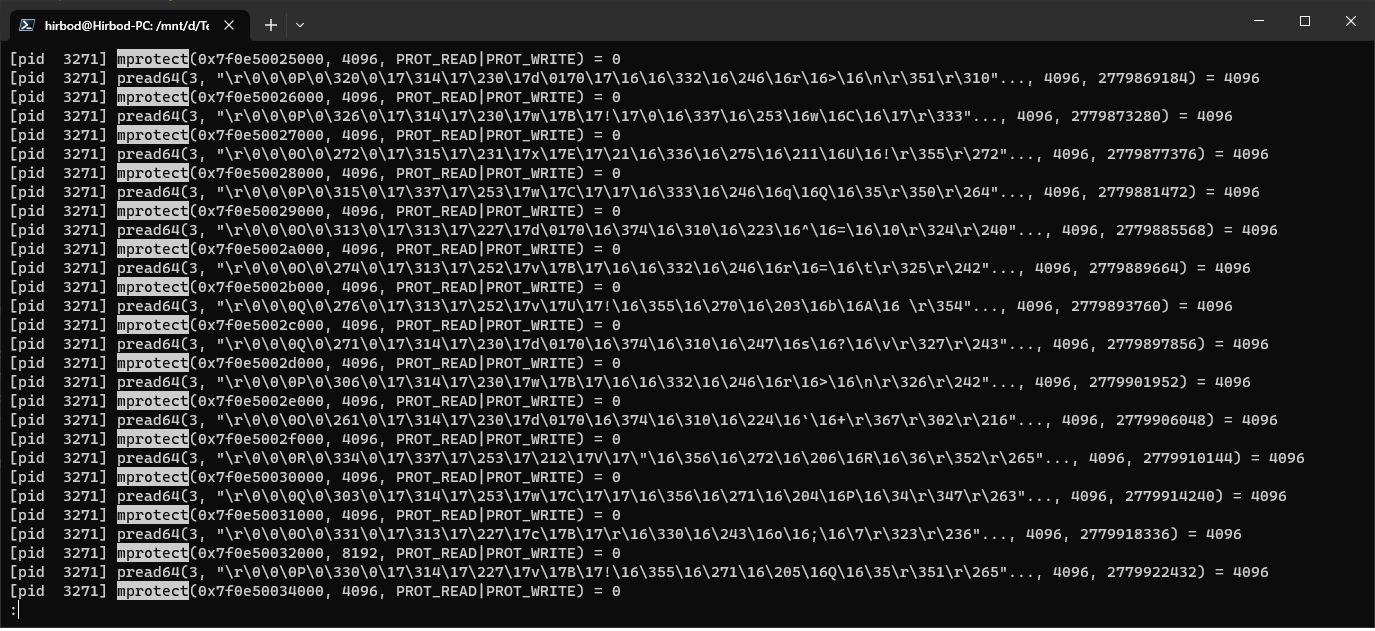
\includegraphics[scale=0.4]{pictures/sqlite3/results/mprotect.png}
    \caption{\lr{mprotect} در روند اجرای برنامه}
    \label{fig:sqlite3:results:mprotect}
\end{figure}
اما یک نکته‌ی عجیبی وجود داشت. هیچ‌گاه
\codeword{mprotect}
در سورس کد
\lr{sqlite}
صدا زده نمی‌شد!
(شکل \ref{fig:sqlite3:results:mprotect2})
این موضوع ما را به این فرضیه صوق داد که احتمالا این موضوع تقصیر
\codeword{malloc}
است. زمانی که برای بار اول
\codeword{malloc}
صدا زده می‌شود، به جای اینکه یک فضای کمی از حافظه هر بار از سیستم عامل درخواست شود، یک فضای بزرگ
از مموری از سیستم عامل درخواست می‌شود که تمام آن فضا غیر قابل نوشتن و خواندن است.
زمانی که
\codeword{malloc}
صدا زده می‌شود، هر بار بخشی از حافظه به کمک
\codeword{mprotect}
قابل خواندن و نوشتن می‌شود. این موضوع نشان می‌دهد که چرا هم در
\lr{MySQL} و هم \lr{SQlite}
این رفتار که چند دستور
\codeword{mprotect} \lr{batch}
نمی‌شدند را شاهد بودیم.
\begin{figure}[H]
    \centering
    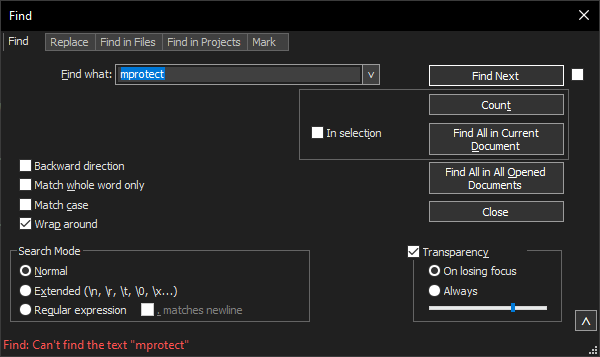
\includegraphics[scale=0.6]{pictures/sqlite3/results/mprotect2.png}
    \caption{وجود نداشتن \lr{mprotect} در سورس کد sqlite}
    \label{fig:sqlite3:results:mprotect2}
\end{figure}
یک نکته‌ی دیگر که می‌توان به آن توجه کرد این است که با اینکه صرفا تعداد ترد‌ها در ماشین
مجازی نصف شده بودند ولی با این حال
\lr{TPM}
ما تقریبا یک چهارم شد. با کمی توجه متوجه می‌شویم که تعداد
\lr{TLB miss}های
ما از حدود ۱۰ میلیون در محیط
\lr{bare metal}
به حدود
100 میلیون رسیده است!
این موضوع به احتمال خیلی زیاد دلیل افت به شدت بالای
\lr{TPM}
است. یعنی انتظار داشتیم که سرعت به خاطر کمتر شدن تعداد هسته‌ها و ترد‌ها حدودا نصف
(و شاید کمتر از نصف چرا که برنامه \lr{io intensive} است)
شود ولی حدودا ۴ برابر بدتر شد عملکرد دیتابیس. نکته‌ی دیگری که باید به آن توجه کرد این است که
در اینجا
\lr{TLB shootdown}
هم نداریم و کلا تعداد آنها در اردر ۲۰ است.

یک نکته‌ی دیگر که نیز به کارکرد
\lr{SQlite}
بر می‌گردد این است که اگر دقت کنید متوجه می‌شوید که تعداد
\lr{pread64}
به شدت بالاست و حدود ۱۰۰۰ برابر بیشتر از
\lr{pwrite64}
است. این موضوع به احتمال خوبی برای این مورد است که
\lr{SQlite}
چیزی را در مموری
\lr{cache}
نمی‌کند. در عوض مجبور است که برای همین موضوع کلی در فایل جلو و عقب برود که جایی
که نیاز به نوشتن دارد را پیدا کند. این موضوع دلیلی است که
\lr{SQlite}
فقط برای داده‌های کوچک خوب است.